To visualize the a hologenic architecture different tasks are introduced. In the blackboard node, an area is set with subsections.
On each sections there are different tasks to be exectuted. 

To start the hologenic architecture, start the script \textit{1\_AgentController.py}. This will start n \acp{uav} (previously passed as parameter 
when starting the containers). Each \acs{uav} will take on a task, with a small time gap between starting to prevent overlap in task exectutions. 
When a \acs{uav} completed its task it will notify the others it is completed and take on the next available task.


\begin{figure}[ht]
    \centering
    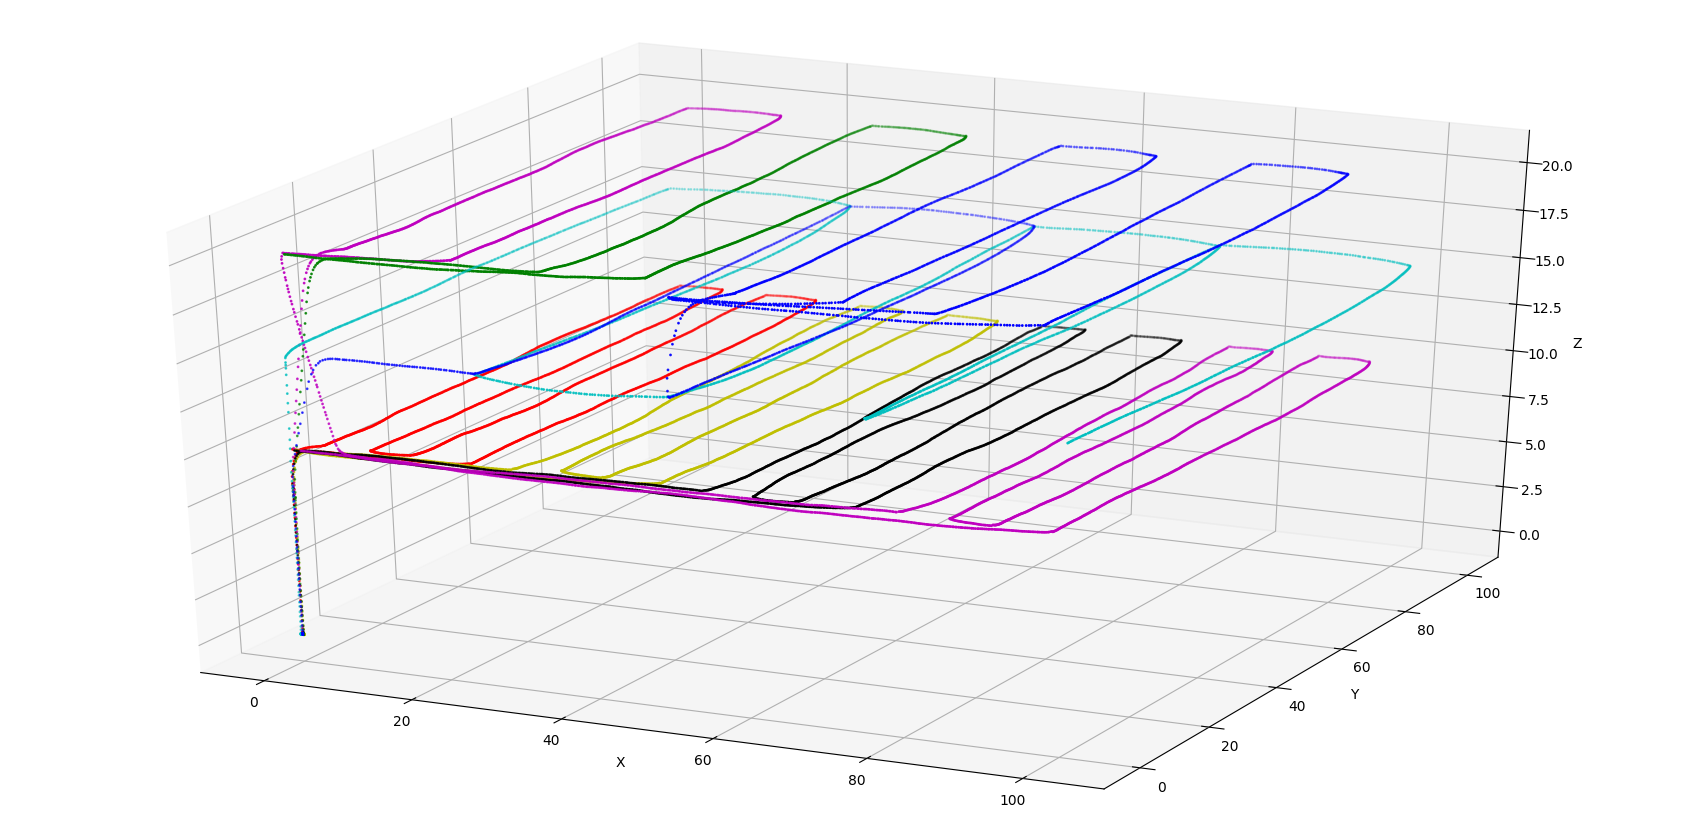
\includegraphics[scale=0.3]{hologenic/hologenicFull.png}
    \caption[hologenic flight patters]{hologenic flight patters\footnotemark.}
\end{figure}

In this example 3 tasks are added in the blackboard, with three different altitudes. Each colors represents a \acs{uav}. 
By giving each task a unique altitude it is easier to visualize 
the completed tasks by a \acs{uav} in combination with the flight pattern for further analysis. 